\documentclass[12pt, a4paper]{article}

\usepackage[hmargin=2.5cm, vmargin=2cm]{geometry}
\usepackage{amsthm, amssymb, mathtools, yhmath, graphicx}
\usepackage{fontspec, type1cm, titlesec, titling, fancyhdr, tabularx}
\usepackage{caption}
\usepackage{color}
\usepackage{hhline}
\usepackage{unicode-math}
\usepackage{nicefrac}

\usepackage[CheckSingle, CJKmath]{xeCJK}
\usepackage{CJKulem}
\usepackage{enumitem}
\usepackage[usenames, dvipsnames]{xcolor}
\usepackage{colortbl}
\usepackage{circuitikz}
%\setCJKmainfont[BoldFont=cwTex Q Hei]{cwTex Q Ming}
%\setCJKsansfont[BoldFont=cwTex Q Hei]{cwTex Q Ming}
%\setCJKmonofont[BoldFont=cwTex Q Hei]{cwTex Q Ming}
\setCJKmainfont[BoldFont=cwTeX Q Hei]{cwTeX Q Ming}

\def\normalsize{\fontsize{12}{18}\selectfont}
\def\large{\fontsize{14}{21}\selectfont}
\def\Large{\fontsize{16}{24}\selectfont}
\def\LARGE{\fontsize{18}{27}\selectfont}
\def\Huge{\fontsize{20}{30}\selectfont}

\titleformat{\section}{\bf\Large}{\arabic{section}}{24pt}{}
\titleformat{\subsection}{\large}{\arabic{subsection}.}{12pt}{}
\titlespacing*{\subsection}{0pt}{0pt}{1.5ex}

\parindent=24pt

\DeclarePairedDelimiter{\abs}{\lvert}{\rvert}
\DeclarePairedDelimiter{\norm}{\lVert}{\rVert}
\DeclarePairedDelimiter{\inpd}{\langle}{\rangle}
\DeclarePairedDelimiter{\ceil}{\lceil}{\rceil}
\DeclarePairedDelimiter{\floor}{\lfloor}{\rfloor}

\newcommand{\unit}[1]{\:(\text{#1})}
\newcommand{\img}{\mathrm{i}}

\title{ \bf {\huge 電子電路實驗4:相位測量}\\ 實驗預報}
\author{B02901178 江誠敏}
\date{2014/09/21}

\begin{document}

\maketitle

\section{實驗目的}
在 AC 電路中,我們可利用示波器來量取兩信號之相位差,本實驗將介紹兩種最常用的相位測量(Phase Measurement)方法:
\begin{enumerate}[itemsep=0pt]
	\item 利薩如圖形法(Lissajous Figures Method)。
	\item 雙軌跡直接測量法(Dual-Trace Direct Measurement Method)。
\end{enumerate}

\section{實驗步驟}
\begin{enumerate}[itemsep=0pt]
	\item 使用LCR 計量測電容值,並用數位電表量測電阻值。
	\item 連接RC電路如下圖。
	\item 調整示波器於X-Y mode,將不同sin波頻率(100Hz/200Hz/500Hz/1kHz/2kHz/5kHz/10kHz)得到的Lissajous figure記錄下來,並計算$V_c$與$V_s$間之相位差。
	\item 調整示波器於Dual-Trace mode,將不同sin波頻率得到的$V_c$與$V_s$記錄下來,並觀察$V_c$與$V_s$間之相位差。
\end{enumerate}

\begin{center}
	\begin{tikzpicture}[american voltages, scale=1]
		\draw[color=black, thick]
		(0, 0) to [V=$V_s$] (0, 6) 
		(0, 6) to [R, l=$R$] (6, 6) 
		(6, 6) to [C, v=$V_c$] (6, 0)
		(6, 0) to [short] (0, 0)
		(3, 0) node[ground]{}
		;
	\end{tikzpicture}
\end{center}


\section{預報問題}

\begin{enumerate}[itemsep=20pt, topsep=10pt]
	\item {\large 請推導圖中$V_c$與$V_s$相位差之理論值。} \\[10pt]
		假設交流電的頻率是$\omega$,則電阻和電容的阻抗分別為$R, \img \omega C$。則由分壓定率可以知道
		\[ V_s = \frac{1/\img \omega C}{R + 1/\img \omega C} V_s = \frac{1}{1 + \img \omega R C} V_s \]
		因此相位差等於$- \arctan \dfrac{ \omega R C}{1} = - \arctan \omega R C$。

	\item {\large 如何利用利薩如圖形求得兩個頻率相同波形的相位差?請推導之。} \\[10pt]
		假設兩個信號的波形分別為$ x(t) = \cos \omega t , y(t) = \cos \left( \omega t + \phi \right) $,其中$\phi$是兩個的相位差,他們的利薩如圖形為曲線$\gamma(t) = (x(t), y(t))$。\\
		做作標轉換$(\hat{x}, \hat{y}) \rightarrow (\hat{x}', \hat{y}')$,其中
		\[ \hat{x}' = \frac{\hat{x} + \hat{y}}{2}, \: \hat{y}' = \frac{ - \hat{x} + \hat{y} }{2} \]
		容易計算$(\hat{x}, \hat{y})$到$(\hat{x}', \hat{y}')$的座標轉換矩陣為
		\[
			A = \begin{bmatrix}
				1 & 1 \\
				-1 & 1\\
			\end{bmatrix}
		\]
		因此如果$\gamma$在新的座標系的參數式為$\gamma'(t) = (x'(t), y'(t))$,計算得知
		\begin{align*}
			\gamma'(t) &= A \gamma = A (\cos (\omega t), \cos (\omega t + \phi)) \\
			&= \left(\cos (\omega t) (1 + \cos \phi) - \sin (\omega t) \sin \phi, \cos(\omega t) (-1 + \cos \phi) - \sin (\omega t) \sin \phi \right)\\
			&= \left(\alpha \left( \cos (\omega t) \frac{1 + \cos \phi}{\alpha} - \sin (\omega t) \frac{\sin \phi}{\alpha}\right), \beta \left( \cos (\omega t) \frac{-1 + \cos \phi}{\beta} - \sin (\omega t) \frac{\sin \phi}{\beta}\right) \right)
		\end{align*}
		其中$\alpha, \beta$為和差化積因子,計算得知$\alpha = \sqrt{2 + 2\cos \phi)}, \beta = \sqrt{2 - 2\cos \phi}$,並且$\left((1 + \cos \phi) / \alpha \right) ^2 + \left((1 - \cos \phi) / \beta \right) ^2 = 1$,因此可以寫成
		\[
			\gamma'(t) = (\alpha \cos(\omega t + \psi), \beta \sin(\omega t + \psi)), \; \psi = \arccos \left( \frac{1 + \cos \phi }{ \alpha } \right) 
		\]
		也就是說利薩如圖形在原座標上是一個橢圓,兩軸分別在$x = y$和$x = -y$兩直線上,並且長度比為$\sqrt{1 + \cos \phi} : \sqrt{1 - \cos \phi}$。因此量測這兩個長度的比就可以得出相位差,但利薩如圖形似乎難以判斷$\phi$的正負號。

	\item {\large 請利用PSpice或者其他電路模擬軟體模擬上圖之電路,繪出在$V_s$頻率為100Hz、1kHz、以及10kHz下的利薩如圖形。} \\[10pt]

		\begin{figure}[H]
			\centering
			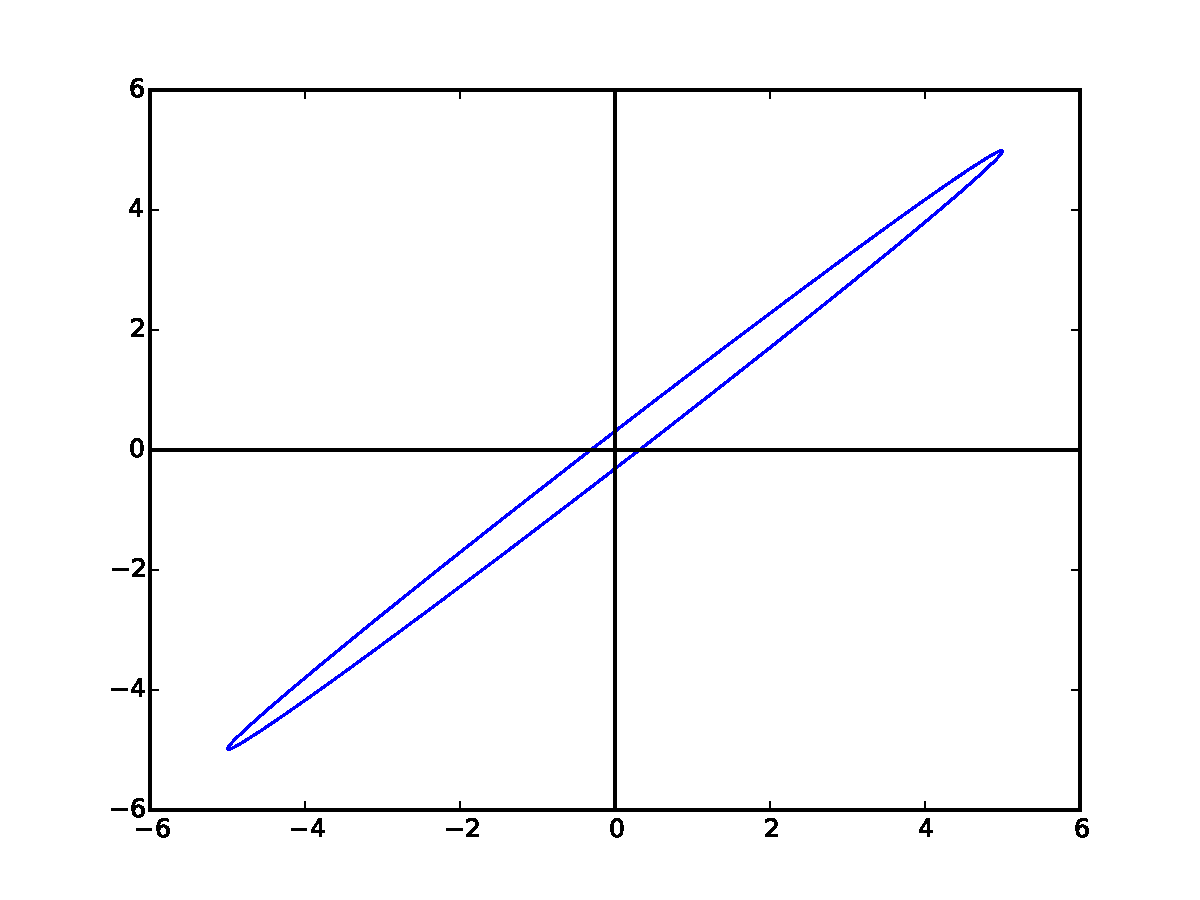
\includegraphics[width=0.6\textwidth]{p100.pdf}
			\caption{100Hz的利薩如圖形}
		\end{figure}
		\begin{figure}[H]
			\centering
			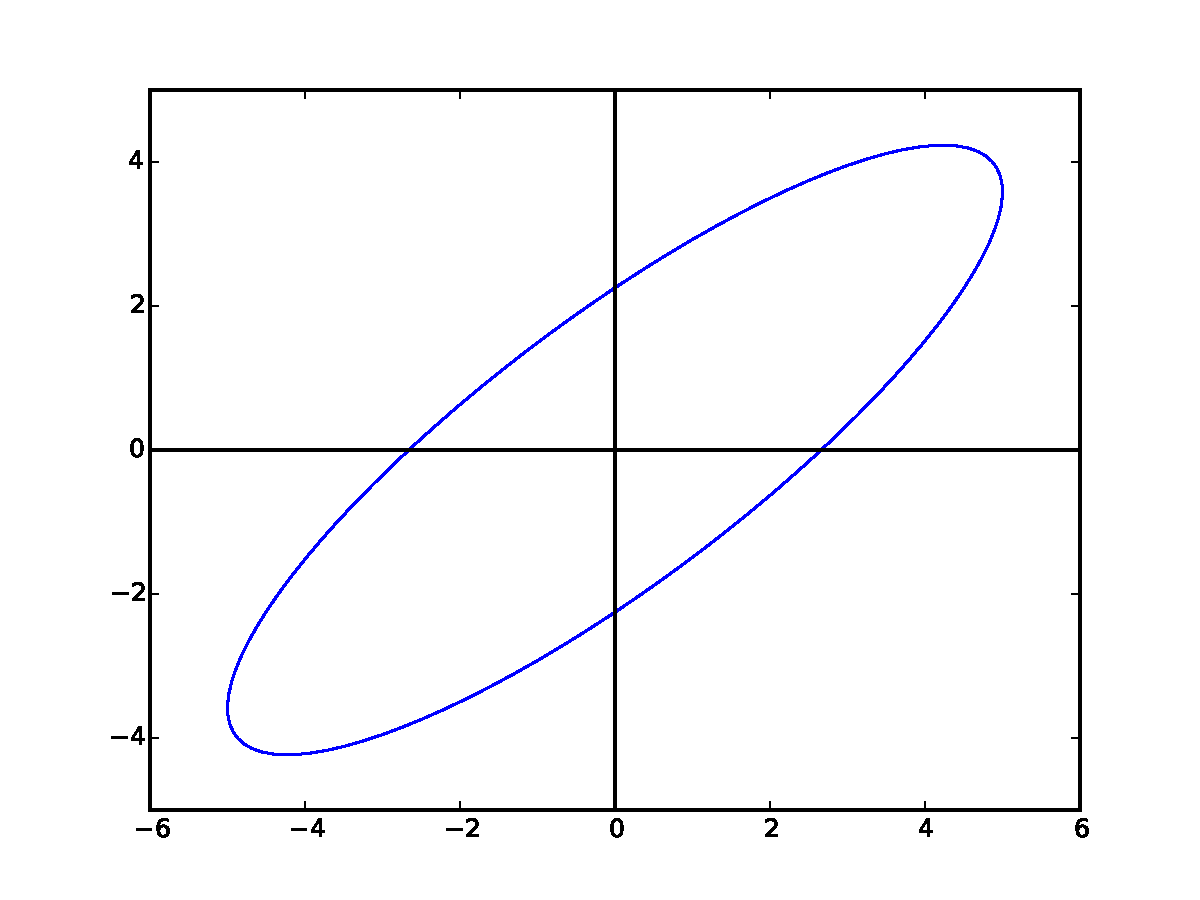
\includegraphics[width=0.6\textwidth]{p1000.pdf}
			\caption{1000Hz的利薩如圖形}
		\end{figure}
		\begin{figure}[H]
			\centering
			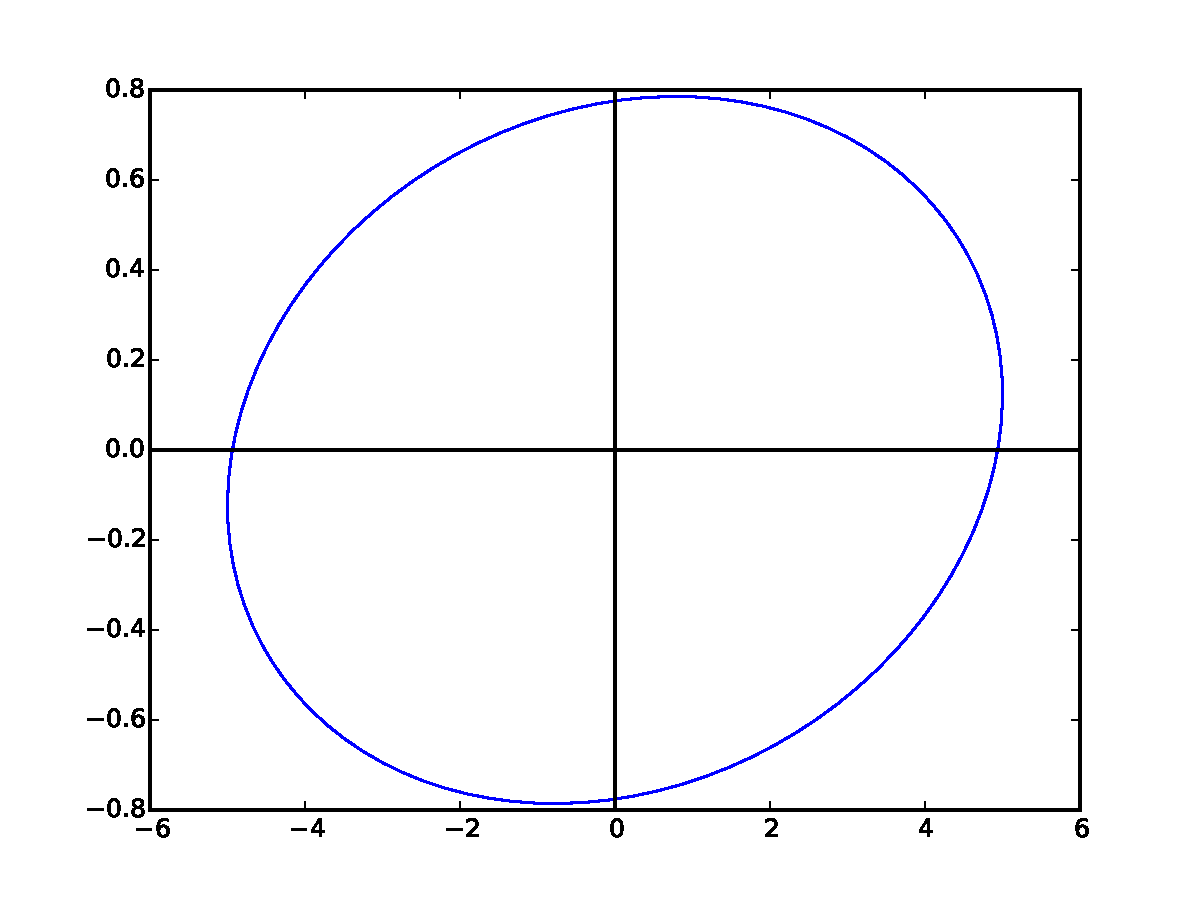
\includegraphics[width=0.6\textwidth]{p10000.pdf}
			\caption{10000Hz的利薩如圖形}
		\end{figure}
		

	\end{enumerate}

	\end{document}

